\documentclass[sigconf,nonacm]{acmart}

\title{Revisiting VulRepair: A Reproduction and Evaluation of T5-based Software Vulnerability Repair Models}

\author{Yushika}
\affiliation{% 
  \institution{University of Ottawa}
  \city{Ottawa}
  \country{Canada}
}
\email{pjhun035@uottawa.ca}

\author{Rina Osman}
\affiliation{% 
  \institution{University of Ottawa}
  \city{Ottawa}
  \country{Canada}
}
\email{rosma012@uottawa.ca}

\author{Olena Naim}
\affiliation{% 
  \institution{University of Ottawa}
  \city{Ottawa}
  \country{Canada}
}
\email{onaim017@uottawa.ca}

\author{Professor Paria Shirani}
\affiliation{% 
  \institution{University of Ottawa}
  \city{Ottawa}
  \country{Canada}
}
\email{pshirani@uottawa.ca}

\renewcommand{\shortauthors}{Jhundoo et al.}

\begin{document}

\begin{abstract}
We revisit and replicate the VulRepair study, a T5-based neural machine translation model designed to automatically repair software vulnerabilities. We re-implement all ten model variants and conduct a comprehensive evaluation to investigate four key research questions (RQs): model accuracy (RQ1), impact of pre-training (RQ2), benefits of BPE tokenization (RQ3), and the contribution of each VulRepair component (RQ4). Through model replication and dataset deduplication, we assess how each design choice contributes to model performance. Our findings confirm the original study's conclusions and further reveal how duplications in the dataset can influence reported accuracy. This study contributes reproducibility insights and extends the VulRepair evaluation to all 10 variants using deduplicated data.
\end{abstract}

\keywords{Vulnerability Repair, T5, Transformer, Dataset Deduplication, Neural Machine Translation, Software Engineering, Reproducibility}

\maketitle

\section{Introduction}
This paper revisits VulRepair, a T5-based model for fixing software vulnerabilities~\cite{vulrepair}. We aim to reproduce the original results and explore additional aspects like deduplication and architecture variations.


\section{Background and Motivation}
Machine learning has recently gained attention in program repair. VulRepair stands out for using a T5 architecture and token-based translation to patch buggy code snippets automatically.


\section{VulRepair Architecture}
The VulRepair architecture is based on T5 and treats vulnerability repair as a translation task. We discuss the tokenizer, pre-training strategies, and model variants.


\section{Methodology}
We replicated all ten models using the original paper’s codebase. We also deduplicated the dataset to study its effect on evaluation. All models were run under the same experimental conditions.


\section{Results}
We report results for all models on both the original and deduplicated datasets. Our findings show performance differences depending on tokenization, pre-training, and architecture.

\paragraph{(RQ4):} What are the contributions of the components of our \textbf{VulRepair}?

To answer this research question, we conducted an ablation study to evaluate the contribution of each component in our \textbf{VulRepair} system (Pre-training + BPE + T5), using models trained exclusively on the deduplicated dataset. We compared VulRepair against a baseline T5 model (No Pre-training + Word-level + T5), systematically varying the components to isolate their individual impact.

Specifically, we evaluated four model variants based on two factors—pre-training and tokenizer type—resulting in the following configurations:

\begin{itemize}
    \item \textbf{Pre-training + BPE + T5 (VulRepair)}: A pre-trained T5 model using Byte-Pair Encoding (BPE).
    \item \textbf{Pre-training + Word-level + T5}: A pre-trained T5 model with a word-level tokenizer.
    \item \textbf{No Pre-training + BPE + T5}: A T5 model without pre-training but using BPE.
    \item \textbf{No Pre-training + Word-level + T5}: A T5 model without pre-training and using a word-level tokenizer.
\end{itemize}

\begin{figure}[H]
    \centering
    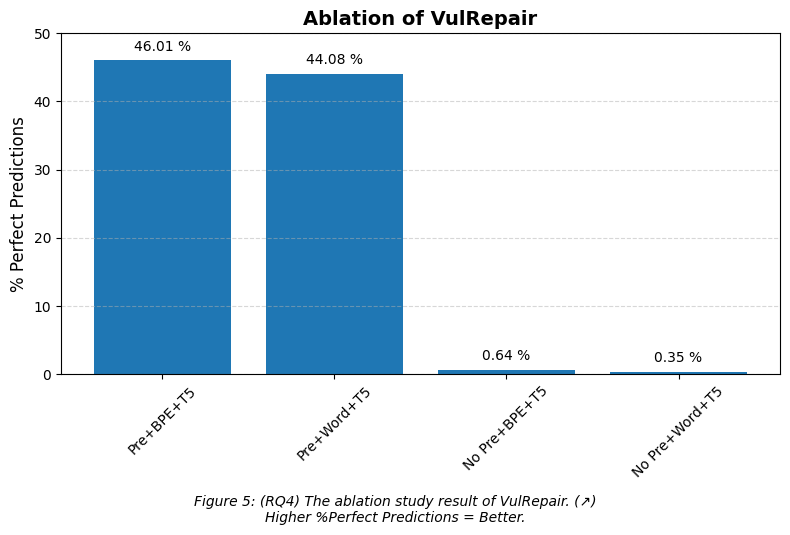
\includegraphics[width=\linewidth]{figures/rq4ablations.png}
    \label{fig:vulrepair_ablation}
\end{figure}


All variants were evaluated using the same metric: \textbf{\% Perfect Predictions}.

Result.
Figure 5 presents the ablation study conducted on the deduplicated dataset to evaluate the contributions of each component in our \textbf{VulRepair}. The results indicate that the pre-training component is the most impactful. When comparing the models with and without pre-training while keeping the BPE tokenizer fixed (Pre+BPE+T5 vs. No Pre+BPE+T5), the \%Perfect Predictions dropped from 46.01\% to 0.64\%, revealing a performance loss of approximately 45.37 percentage points.

The tokenization strategy also contributes meaningfully to the model’s effectiveness. Changing the tokenizer from BPE to word-level while keeping pre-training enabled (Pre+BPE+T5 vs. Pre+Word+T5) led to a slight reduction from 46.01\% to 44.08\%, a drop of 1.93 percentage points.

Most notably, in the absence of both pre-training and BPE tokenization (No Pre+Word+T5), the performance plummets to just 0.35\%, emphasizing the necessity of both components. These findings highlight that designing a robust Transformer-based automated vulnerability repair system like VulRepair demands not only architectural depth, but also careful attention to pre-training and tokenization strategies in order to achieve high prediction accuracy.

\section{Discussion}
Our replication confirms many claims made by the original authors. However, dataset duplication significantly impacts accuracy metrics and should be considered in future evaluations.



\begin{figure}[H]
    \begin{center}
    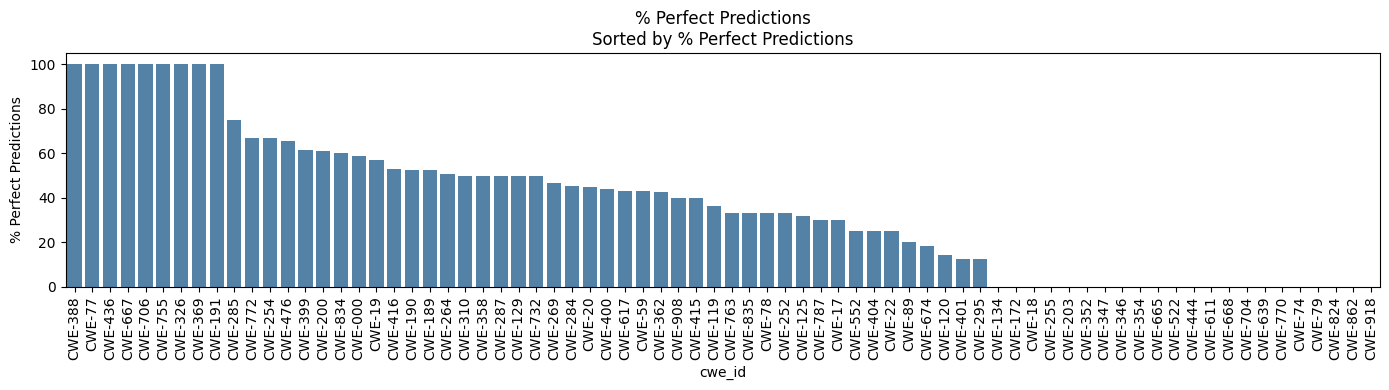
\includegraphics[width=1\linewidth]{figures/cve.png}
    \end{center}
    \begin{center}
        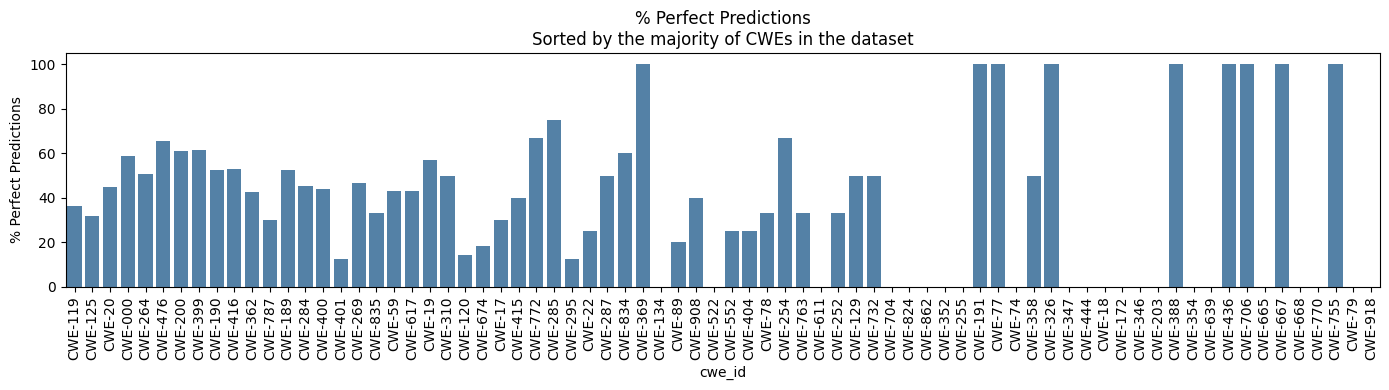
\includegraphics[width=1\linewidth]{figures/cwe.png}
    \end{center}
    \caption{(Discussion) The \%Perfect Predictions (y-axis) of our \textbf{VulRepair} according to each type of CWE (x-axis, sorted by \% perfect predictions and sorted by the majority of CWEs in the dataset). Detailed statistic can be found in Appendix.}
    \label{fig:cve}
\end{figure}



\section{Related Work}
Several other works explore machine learning-based vulnerability repair, including CodeBERT and CURE. We compare these with VulRepair in terms of methodology and reported performance.


\section{Threats to Validity}
Threats include implementation differences, reproducibility limitations, and dataset preprocessing choices that could affect our results.


\section{Conclusion}
We successfully reproduced VulRepair, evaluated all 10 model variants, and introduced deduplication to better understand the reliability of reported performance.


\bibliographystyle{ACM-Reference-Format}
\bibliography{sample-base}

\end{document}
